\begin{figure}[htb]
\centering
\includegraphics[page=6,width=0.33\textwidth]{\FCNCFigures/xTFW/showFake/NOMINAL/reg2mtau1b2jos/tautaumass.pdf}
\put(-30, 80){\textbf{(a1)}}
\includegraphics[page=6,width=0.33\textwidth]{\FCNCFigures/xTFW/showFake/NOMINAL/reg2mtau1b2jos/ttvismass.pdf}
\put(-30, 80){\textbf{(a2)}}
\includegraphics[page=6,width=0.33\textwidth]{\FCNCFigures/xTFW/showFake/NOMINAL/reg2mtau1b2jos/t1mass.pdf}
\put(-70, 70){\textbf{(a3)}}
\\
\includegraphics[page=6,width=0.33\textwidth]{\FCNCFigures/xTFW/showFake/NOMINAL/reg2mtau1b3jos/tautaumass.pdf}
\put(-30, 80){\textbf{(b1)}}
\includegraphics[page=6,width=0.33\textwidth]{\FCNCFigures/xTFW/showFake/NOMINAL/reg2mtau1b3jos/ttvismass.pdf}
\put(-30, 80){\textbf{(b2)}}
\includegraphics[page=6,width=0.33\textwidth]{\FCNCFigures/xTFW/showFake/NOMINAL/reg2mtau1b3jos/drtautau.pdf}
\put(-70, 70){\textbf{(b3)}}
\\
\includegraphics[page=6,width=0.33\textwidth]{\FCNCFigures/tthML/showFake/faketau/postfit/NOMINAL/reg1l2tau1bnj_os/ttvismass.pdf}
\put(-30, 80){\textbf{(c1)}}
\includegraphics[page=6,width=0.33\textwidth]{\FCNCFigures/tthML/showFake/faketau/postfit/NOMINAL/reg1l2tau1bnj_os/drtautau.pdf}
\put(-30, 80){\textbf{(c2)}}
\includegraphics[page=6,width=0.33\textwidth]{\FCNCFigures/tthML/showFake/faketau/postfit/NOMINAL/reg1l2tau1bnj_os/t2vismass.pdf}
\put(-70, 70){\textbf{(c3)}}
\\
\caption{ The BDT input distributions for the background and merged signal in the STH $\thadhad$ (a1-3), TTH $\thadhad$ (b1-3),  $l\thadhad$ (c1-3) channels. }% The Kolmogorov Test values for the training and testing BDT distributions are also indicated.
\label{fig:mva_input}
\end{figure}

\begin{figure}[htb]
\centering
\includegraphics[page=6,width=0.33\textwidth]{\FCNCFigures/tthML/showFake/fakelep/postfit/NOMINAL/reg2lSS1tau1bnj_os/t2vismass.pdf}
\put(-30, 80){\textbf{(11)}}
\includegraphics[page=6,width=0.33\textwidth]{\FCNCFigures/tthML/showFake/fakelep/postfit/NOMINAL/reg2lSS1tau1bnj_os/drtautau.pdf}
\put(-30, 80){\textbf{(12)}}
\includegraphics[page=6,width=0.33\textwidth]{\FCNCFigures/tthML/showFake/fakelep/postfit/NOMINAL/reg2lSS1tau1bnj_os/drtaujmin.pdf}
\put(-70, 70){\textbf{(13)}}
\\
\includegraphics[page=6,width=0.33\textwidth]{\FCNCFigures/tthML/showFake/faketau/postfit/NOMINAL/reg1l1tau1b2j_os/drtautau.pdf}
\put(-30, 80){\textbf{(b1)}}
\includegraphics[page=6,width=0.33\textwidth]{\FCNCFigures/tthML/showFake/faketau/postfit/NOMINAL/reg1l1tau1b2j_os/tau_pt_0.pdf}
\put(-30, 80){\textbf{(b2)}}
\includegraphics[page=6,width=0.33\textwidth]{\FCNCFigures/tthML/showFake/faketau/postfit/NOMINAL/reg1l1tau1b2j_os/ttvismass.pdf}
\put(-70, 70){\textbf{(b3)}}
\\
\includegraphics[page=6,width=0.33\textwidth]{\FCNCFigures/tthML/showFake/faketau/postfit/NOMINAL/reg1l1tau1b3j_os/ttvismass.pdf}
\put(-30, 80){\textbf{(c1)}}
\includegraphics[page=6,width=0.33\textwidth]{\FCNCFigures/tthML/showFake/faketau/postfit/NOMINAL/reg1l1tau1b3j_os/tau_pt_0.pdf}
\put(-30, 80){\textbf{(c2)}}
\includegraphics[page=6,width=0.33\textwidth]{\FCNCFigures/tthML/showFake/faketau/postfit/NOMINAL/reg1l1tau1b3j_os/drtautau.pdf}
\put(-70, 70){\textbf{(c3)}}
\\
\caption{STH $\tlhad$ (a1-3),TTH $\tlhad$ (b1-3),$2lSS\tauhad$ (c1-3)道的本底和信号BDT输入变量的分布的对比 }% The Kolmogorov Test values for the training and testing BDT distributions are also indicated.
\label{fig:mva_input}
\end{figure}